%!Tex Root = ../Main.tex
% ./Packete_und_Deklarationen.tex
% ./Titlepage.tex
% ./Motivation.tex
% ./Implementierung1_Tables_DT_AST.tex,
% ./Implementierung2_Pntr_Array.tex,
% ./Implementierung3_Struct_Derived.tex,
% ./Implementierung4_Fun.tex,
% ./Ergebnisse_und_Ausblick.tex

\chapter{Einführung}
\label{ch:einführung}

\section{Compiler und Interpreter}
Der wohl wichtigsten zu klärenden Begriffe, sind die eines \colorbold{Compilers} (Definition~\ref{def:compiler}) und eines  \colorbold{Interpreters} (Definition~\ref{def:interpreter}), da das Schreiben eines Compilers von der \colorbold{PicoC-Sprache} $L_{PicoC}$ in die \colorbold{RETI-Sprache} $L_{RETI}$ das Thema dieser Bachelorarbeit ist und die Definition eines \colorbold{Interpreters} genutzt wird, um zu definieren was ein \colorbold{Compiler} ist. Des Weiteren wurde zur \colorbold{Qualitätsicherung} ein \colorbold{RETI-Interpreter} implementiert, um mithilfe des \colorbold{GCC}\footnote{Sammlung von Compilern für Linux bzw. GNU-Linux, steht für \colorbold{G}NU \colorbold{C}ompiler \colorbold{C}ollection} und von \colorbold{Tests} die \colorbold{Beziehungen} in \ref{eq:compiler_beziehungen} zu belegen (siehe Subkapitel~\ref{sec:qualitätssicherung}).

\begin{Definition}{Interpreter}{interpreter}
  \colorbold{Interpretiert} die \colorbold{Instructions} bzw. \colorbold{Statements} eines Programmes $P$ direkt.

  Auf die Implementierung bezogen arbeitet ein Interpreter auf den compilerinternen \colorbold{Sub-Bäumen} des \colorbold{Abstract Syntax Tree} (Definition~\ref{def:abstrakte_syntax_tree}) und führt je nach Komposition der \colorbold{Nodes} des Abstract Syntax Tree, auf die er während des Darüber-Iterierens stösst unterschiedliche Anweisungen aus.\footcite{g_siek_course_2022}
\end{Definition}

% https://tex.stackexchange.com/questions/51228/how-to-increase-the-horizontal-distance-between-nodes
\begin{Definition}{Compiler}{compiler}
  \colorbold{Kompiliert} ein Program $P_1$, welches in einer Sprache $L_1$ geschrieben ist, in ein Program $P_2$, welches in einer Sprache $L_2$ geschrieben ist.

  Wobei \colorbold{Kompilieren} meint, dass das Program $P_1$ so in das Program $P_2$ übersetzt wird, dass bei beiden Programmen, wenn sie von \colorbold{Interpretern} ihrer jeweiligen Sprachen $L_1$ und $L_2$ \colorbold{interpretiert} werden, der gleiche \colorbold{Output} rauskommt. Also beide Programme $P_1$ und $P_2$ die gleiche \colorbold{Semantik} haben und sich nur \colorbold{syntaktisch} durch die Sprachen $L_1$ und $L_2$, in denen sie geschrieben stehen unterscheiden.\footcite{g_siek_course_2022}

  % https://tex.stackexchange.com/questions/233615/change-equation-number-latex
  % https://tex.stackexchange.com/questions/245979/numberwithinequationsubsection-fails-for-subsections-0
  \numberwithin{equation}{\tcbcounter}
  \begin{equation}
    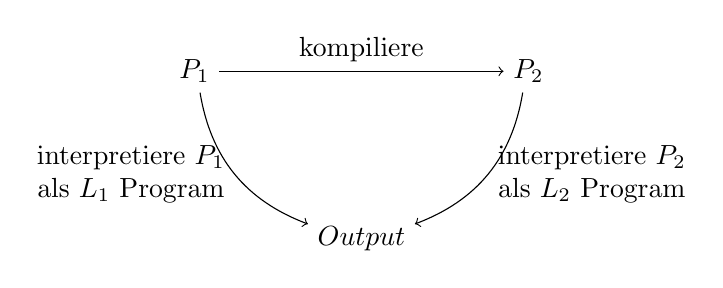
\begin{tikzpicture}[auto, baseline=(current  bounding  box.center)]
      \node (program1) at (135:3) {$P_{1}$};
      \node (program2) at (45:3) {$P_{2}$};
      \node (output)  at (270:0) {$Output$};

      % https://tex.stackexchange.com/questions/24372/how-to-add-newline-within-node-using-tikz
      \draw[->] (program1) to node[above] {kompiliere} (program2);
      \draw[->] (program1) to[bend right] node[left, align=center] {interpretiere $P_{1}$\\ als $L_{1}$ Program} (output);
      \draw[->] (program2) to[bend left] node[right, align=center] {interpretiere $P_{2}$\\ als $L_{2}$ Program} (output);
    \end{tikzpicture}
    \label{eq:compiler_beziehungen}
  \end{equation}
\end{Definition}

\begin{Special_Paragraph}
  Im Folgenden wird ein voll ausgeschriebener \colorbold{Compiler} als $C_{i\_w\_k\_{min}}^{o\_j}$ geschrieben, wobei $C_w$ die \colorbold{Sprache} bezeichnet, die der Compiler als \colorbold{Input} nimmt und zu einer nicht näher spezifizierten Maschienensprache $L_{B_i}$ einer Maschiene $M_i$ kompiliert. Fall die Notwendigkeit besteht die \colorbold{Maschiene} $M_i$ anzugeben, zu dessen \colorbold{Maschienensprache} $L_{B_i}$ der Compiler kompiliert, wird das als $C_{i}$ geschrieben. Falls die Notwendigkeit besteht die \colorbold{Sprache} $L_o$ anzugeben, in der der Compiler selbst geschrieben ist, wird das als $C^o$ geschrieben. Falls die Notwendigkeit besteht die Version der Sprache, in die der Compiler kompiliert ($L_{w\_k}$) oder in der er selbst geschrieben ist ($L_{o\_j}$) anzugeben, wird das als $C_{w\_k}^{o\_j}$ geschrieben. Falls es sich um einen \colorbold{minimalen Compiler} handelt (Definition~\ref{def:minimaler_compiler}) kann man das als $C_{min}$ schreiben.
\end{Special_Paragraph}

Üblicherweise kompiliert ein \colorbold{Compiler} ein \colorbold{Program}, dass in einer \colorbold{Programmiersprache} geschrieben ist zu \colorbold{Maschienenncode}, der in \colorbold{Maschienensprache} (Definition~\ref{def:maschienensprache}) geschrieben ist, aber es gibt z.B. auch \colorbold{Transpiler} (Definition~\ref{def:transpiler}) oder \colorbold{Cross-Compiler} (Definition~\ref{def:cross_compiler}). Des Weiteren sind \colorbold{Maschienensprache} und \colorbold{Assemblersprache} (Definition~\ref{def:assemblersprache}) voneinander zu unterscheiden.

\begin{Definition}{Maschienensprache}{maschienensprache}
  Programmiersprache, deren mögliche Programme die \colorbold{hardwarenaheste Repräsentation} eines möglicherweise zuvor hierzu kompilierten bzw. assemblierten Programmes darstellen. Jeder Maschienenbefehl entspricht einer bestimmten \colorbold{Aufgabe}, die die CPU im \colorbold{vereinfachten Fall} in einem \colorbold{Zyklus} der \colorbold{Fetch-} und \colorbold{Execute-Phase}, genauergesagt in der \colorbold{Execute-Phase} übernehmen kann oder allgemein in einer \colorbold{geringen konstanten} Anzahl von Fetch- und Execute Phasen im \colorbold{komplexeren Fall}. Die Maschienenbefehle sind meist so designed, dass sie sich innerhalb bestimmter \colorbold{Wortbreiten}, die $2$er Potenzen sind codieren lassen. Im einfachsten Fall innerhalb einer \colorbold{Speicherzelle} des \colorbold{Hauptspeichers}.\footnote{Viele Prozessorarchitekturen erlauben es allerdings auch z.B. \colorbold{zwei} Maschienenbefehle in \colorbold{eine} Speicherzelle des Hauptspeichers zu komprimieren, wenn diese zwei Maschienenbefehle keine Operanden mit zu großen \colorbold{Immediates} (Definition~\ref{def:immediate}) haben.}\footcite{scholl_betriebssysteme_2020}
\end{Definition}

\begin{Definition}{Assemblersprache (bzw. engl. Assembly Language)}{assemblersprache}
  Eine sehr \colorbold{hardwarenahe} Programmiersprache, derren \colorbold{Instructions} eine starke Entsprechung zu bestimmten Maschienenbefehlen bzw. Folgen von Maschienenbefehlen\footnote{Instructions der Assemblersprache, die mehreren Maschienenbefehlen entsprechen werden auch als \colorbold{Pseudo-Instructions} bezeichnet und entsprechen dem, was man im allgemeinen als Macro bezeichnet.} haben.
  Viele \colorbold{Instructions} haben eine ähnliche übliche Struktur \verb|Operation <Operanden>|, mit einer \colorbold{Operation}, die einem \colorbold{Opcode} eines Maschienenbefehls bezeichnet und keinen oder mehreren \colorbold{Operanden}, wie die späteren Maschienenbefehle, denen sie entsprechen. Allerdings gibt es oftmals noch viel \glqq syntaktischen Zucker\grqq\; innerhalb\footnote{Z.B. erlaubt die Assemblersprache des \colorbold{GCC} für die \colorbold{$X_{86\_64}$-Architektur} für manche Operanden die Syntax \smalltt{n(\%r)}, die einen \colorbold{Speicherzugriff} mit \colorbold{Offset} $n$ zur Adresse, die im \colorbold{Register} \smalltt{\%r} steht durchführt, wobei z.B. die Klammern \smalltt{()} usw. nur \glqq syntaktischer Zucker\grqq sind und natürlich nicht mitcodiert werden.} der Instructions und drumherum\footnote{Z.B. sind im $X_{86\_64}$ Assembler die Instructions in \colorbold{Blöcken} untergebracht, die ein \colorbold{Label} haben und zu denen mittels  \smalltt{jmp <label>} gesprungen werden kann. Ein solches Konstrukt, was vor allem auch noch relativ beliebig wählbare Bezeichner verwendet hat keine direkte Entsprechung in einem handelsüblichen Prozessor und Hauptspeicher.}.\footcite{scholl_einfuhrung_2021}
\end{Definition}

Ein \colorbold{Assembler} (Definition~\ref{def:assembler}) ist in üblichen Compilern in einer bestimmten Form meist schon integriert sein, da Compiler üblicherweise direkt \colorbold{Maschienencode} bzw. \colorbold{Objectcode} (Definition~\ref{def:objectcode}) erzeugen. Ein \colorbold{Compiler} soll möglichst viel von seiner internen Funktionsweise und der damit verbundenen Theorie für den Benutzer abstrahieren und dem Benutzer daher standardmäßig einfach nur den Output liefern, den er in den allermeisten Fällen haben will, nämlich den \colorbold{Maschienencode} bzw. \colorbold{Objectcode}, der direkt ausführbar ist bzw. wenn er später mit dem \colorbold{Linker} (Definition~\ref{def:linker}) zu Maschiendencode zusammengesetzt wird ausführbar ist.

\begin{Definition}{Assembler}{assembler}
  Übersetzt im allgemeinen \colorbold{Assemblercode}, der in \colorbold{Assemblersprache} geschrieben ist zu \colorbold{Maschienencode} bzw. \colorbold{Objectcode} in \colorbold{binärerer Repräsentation}, der in \colorbold{Maschienensprache} geschrieben ist.\footcite{scholl_einfuhrung_2021}
\end{Definition}

\begin{Definition}{Objectcode}{objectcode}
  Bei komplexeren Compilern, die es erlauben den Programmcode in \colorbold{mehrere Dateien} aufzuteilen wird häufig \colorbold{Objectcode} erzeugt, der neben der Folge von Maschienenbefehlen in \colorbold{binärer Repräsentation} auch noch Informationen für den \colorbold{Linker} enthält, die im späteren \colorbold{Maschiendencode} nicht mehr enthalten sind, sobald der \colorbold{Linker} die Objektdateien zum Maschienencode zusammengesetzt hat.\footcite{scholl_einfuhrung_2021}
\end{Definition}

\begin{Definition}{Linker}{linker}
  Programm, dass \colorbold{Objektcode} aus mehreren Objektdateien zu ausführbarem \colorbold{Maschienencode} in eine ausführbare Datei oder Bibliotheksdatei \colorbold{linkt}, sodass unter anderem kein vermeidbarer \colorbold{doppelter} Code darin vorkommt.\footcite{scholl_einfuhrung_2021}
\end{Definition}

Der \colorbold{Maschienencode}, denn ein üblicher Compiler einer Programmiersprache generiert, enthält seine Folge von Maschienenbefehlen üblicherweise in \colorbold{binärer Repräsentation}, da diese in erster Linie für die Maschiene, die binär arbeitet verständlich sein sollen und nicht für den Programmierer.

Der \colorbold{PicoC-Compiler}, der den Zweck erfüllt für Studenten ein \colorbold{Anschauungs- und Lernwerkzeug} zu sein, generiert allerdings Maschienencode, der die Maschienenbefehle bzw. RETI-Befehle in \colorbold{menschenlesbarer Form} mit ausgeschriebenen RETI-Operationen, RETI-Registern und Immediates (Definition~\ref{def:immediate}) enthält. Für den \colorbold{RETI-Interpreter} ist es ebenfalls nicht notwendig, dass der Maschienencode, denn der PicoC-Compiler generiert in binärer Darstellung ist, denn es ist für den RETI-Interpreter ebenfalls leichter diese einfach direkt in menschenlesbarer Form zu interpretieren, da der RETI-Interpreter nur die sichtbare Funktionsweise einer RETI-CPU \colorbold{simulieren} soll und nicht deren mögliche interne Umsetzung\footnote{Eine \colorbold{RETI-CPU} zu bauen, die menschenlesbaren Maschienencode in z.B. \colorbold{UTF-8 Codierung} ausführen kann, wäre dagegen unnötig kompliziert und aufwändig, da Hardware \colorbold{binär} arbeitet und man dieser daher lieber direkt die binär codierten Maschienenbefehle übergibt, anstatt z.B. eine unnötig \colorbold{platzverbrauchenden} UTF-8 Codierung zu verwenden, die nur in sehr vielen Schritt einen Befehl verarbeiten kann, da die Register und Speicherzellen des Hauptspeichers üblicherweise nur \colorbold{32- bzw. 64-Bit Breite} haben.}.

\begin{Definition}{Immediate}{immediate}
  \colorbold{Konstanter Wert}, der als \colorbold{Teil} eines \colorbold{Maschienenbefehls} gespeichert ist und dessen \colorbold{Wertebereich} dementsprechend auch durch die die Anzahl an Bits, die ihm innerhalb dieses \colorbold{Maschienenbefehls} zur Verfügung gestellt sind, \colorbold{beschränkter} ist als bei sonstigen Werten innerhalb des Hauptspeichers, denen eine ganze Speicherzelle des Hauptspeichers zur Verfügung steht.\footcite{ljohhuh_what_2018}
\end{Definition}

\begin{Definition}{Transpiler (bzw. Source-to-source Compiler)}{transpiler}
  Kompiliert zwischen Sprachen, die ungefähr auf dem \colorbold{gleichen} Level an \colorbold{Abstraktion} arbeiten\footnote{Die Programmiersprache \colorbold{TypeScript} will als \colorbold{Obermenge} von \colorbold{JavaScript} die Sprachhe Javascript \colorbold{erweitern} und gleichzeitig die \colorbold{syntaktischen Mittel} von JavaScript unterstützen. Daher bietet es sich Typescript zu Javascript zu \colorbold{transpilieren}.}\footcite{thiemann_compilerbau_2021}
\end{Definition}

\begin{Definition}{Cross-Compiler}{cross_compiler}
  Kompiliert auf einer \colorbold{Maschine} $M_1$ ein Program, dass in einer \colorbold{Sprache} $L_w$ geschrieben ist für eine \colorbold{andere Maschine} $M_2$, wobei beide Maschinen $M_1$ und $M_2$ unterschiedliche \colorbold{Maschienensprachen} $B_1$ und $B_2$ haben.\footnote{Beim \colorbold{PicoC-Compiler} handelt es sich um einen \colorbold{Cross-Compiler} $C_{PicoC}^{Python}$.}\footcite{earley_formalism_1970}
\end{Definition}

Ein \colorbold{Cross-Compiler} ist entweder notwendig, wenn eine Zielmaschine $M_2$ nicht ausreichend \colorbold{Rechenleistung} hat, um ein Programm in der Wunschsprache $L_w$ selbst \colorbold{zeitnah} zu kompilieren oder wenn noch kein Compiler $C_w$ für die \colorbold{Wunschsprache} $L_w$ und andere Programmiersprachen $L_o$, in denen man Programmieren wollen würde existiert, der unter der \colorbold{Maschienensprache} $B_2$ einer Zielmaschine $M_2$ läuft.\footnote{Die an vielen Universitäten und Schulen eingesetzen programmierbaren Roboter von \colorbold{Lego Mindstorms} nutzen z.B. einen \colorbold{Cross-Compiler}, um für den programmierbaren Microcontroller eine \colorbold{C-ähnliche Sprache} in die Maschienensprache des Microcontrollers zu kompilieren, da der Microcontroller selbst nicht genug Rechenleistung besitzt, um ein Programm selbst zeitnah zu kompilieren.}

% Das ist das, was der PicoC-Compiler ist

\subsection{T-Diagramme}
\label{sec:t_diagram}
Um die Architektur von \colorbold{Compilern} und \colorbold{Interpretern} übersichtlich darzustellen eignen sich \colorbold{T-Diagramme}, deren Spezifikation aus dem Paper~\cite{earley_formalism_1970} entnommen ist besonders gut, da diese optimal darauf \colorbold{zugeschnitten} sind die Eigenheiten von Compilern in ihrer Art der Darstellung unterzubringen.

Die \colorbold{Notation} setzt sich dabei aus den \colorbold{Blöcken} für ein Program (Definition~\ref{def:t_diagram_program}), einen Übersetzer (Definition~\ref{def:t_diagram_übersetzer}), einen Interpreter (Definition~\ref{def:t_diagram_interpreter}) und eine Maschiene (Definition~\ref{def:t_diagram_maschiene}) zusammen.

\begin{Definition}{T-Diagram Programm}{t_diagram_program}
  Repräsentiert ein \colorbold{Programm}, dass in der \colorbold{Sprache} $L_1$ geschrieben ist und die \colorbold{Funktion} $f$ berechnet.\footcite{earley_formalism_1970}
  \begin{figure}[H]
    \centering
    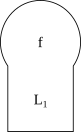
\includegraphics[height=3cm]{./figures/programm.png}
  \end{figure}
\end{Definition}

\begin{Special_Paragraph}
  Es ist bei \colorbold{T-Diagrammen} nicht notwendig beim entsprechenden \colorbold{Platzhalter}, in den man die genutzte \colorbold{Sprache} schreibt, den \colorbold{Namen der Sprache} an ein $L$ dranzuhängen, weil hier immer eine \colorbold{Sprache} steht. Es würde in Definition~\ref{def:t_diagram_program} also reichen einfach eine $1$ hinzuschreiben.
\end{Special_Paragraph}

\begin{Definition}{T-Diagram Übersetzer (bzw. eng. Translator)}{t_diagram_übersetzer}
% TODO: es gilt das Diagram vom Compiler da
  Repräsentiert einen \colorbold{Übersetzer}, der in der \colorbold{Sprache} $L_1$ geschrieben ist und \colorbold{Programme} von der \colorbold{Sprache} $L_2$ in die \colorbold{Sprache} $L_3$ kompiliert.

  Für den \colorbold{Übersetzer} gelten genauso, wie für einen \colorbold{Compiler}\footnote{Zwischen den Begriffen \colorbold{Übersetzung} und \colorbold{Kompilierung} gibt es einen kleinen Unterschied, \colorbold{Übersetzung} ist \colorbold{kleinschrittiger} als \colorbold{Kompilierung} und ist auch zwischen \colorbold{Passes} möglich, \colorbold{Kompilierung} beinhaltet dagegen bereits alle \colorbold{Passes} in einem Schritt. \colorbold{Kompilieren} ist also auch \colorbold{Übsersetzen}, aber \colorbold{Übersetzen} ist nicht immer auch \colorbold{Kompilieren}.} die \colorbold{Beziehungen} in \ref{eq:compiler_beziehungen}.\footcite{earley_formalism_1970}
  \begin{figure}[H]
    \centering
    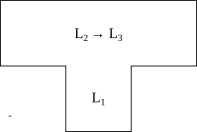
\includegraphics[height=3cm]{./figures/uerbersetzer.png}
  \end{figure}
\end{Definition}

\begin{Definition}{T-Diagram Interpreter}{t_diagram_interpreter}
  Repräsentiert einen \colorbold{Interpreter}, der in der \colorbold{Sprache} $L_1$ geschrieben ist und \colorbold{Programme} in der \colorbold{Sprache} $L_2$ interpretiert.\footcite{earley_formalism_1970}
  \begin{figure}[H]
    \centering
    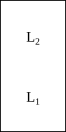
\includegraphics[height=3cm]{./figures/interpreter.png}
  \end{figure}
\end{Definition}

\begin{Definition}{T-Diagram Maschiene}{t_diagram_maschiene}
  Repräsentiert eine \colorbold{Maschiene}, welche ein \colorbold{Programm} in \colorbold{Maschienensprache} $L_1$ ausführt.\footnote{Wenn die Maschiene \colorbold{Programme} in einer höheren Sprache als \colorbold{Maschienensprache} ausführt, ist es auch erlaubt diese Notation zu verwenden, dann handelt es sich um eine \colorbold{Abstrakte Maschiene}, wie z.B. die \colorbold{Python Virtual Machine} (PVM) oder \colorbold{Java Virtual Machine} (JVM).}\footcite{earley_formalism_1970}
  \begin{figure}[H]
    \centering
    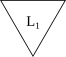
\includegraphics[height=1.5cm]{./figures/machiene.png}
  \end{figure}
\end{Definition}

Aus den verschiedenen \colorbold{Blöcken} lassen sich \colorbold{Kompostionen} bilden, indem man sie \colorbold{adjazent} zueinander platziert. Allgemein lässt sich grob sagen, dass \colorbold{vertikale Adjazents} für \colorbold{Interpretation} und  \colorbold{horinzontale Adjazents} für \colorbold{Übersetzung} steht.

Sowohl \colorbold{horinzontale} als auch \colorbold{vertikale Adjazents} lassen sich, wie man in den Abbildungen \ref{fig:t_diagram_horinzontal_zusammenfassen} und \ref{fig:t_diagram_vertikal_zusammenfassen} erkennen kann zusammenfassen.

\begin{figure}[H]
  \centering
  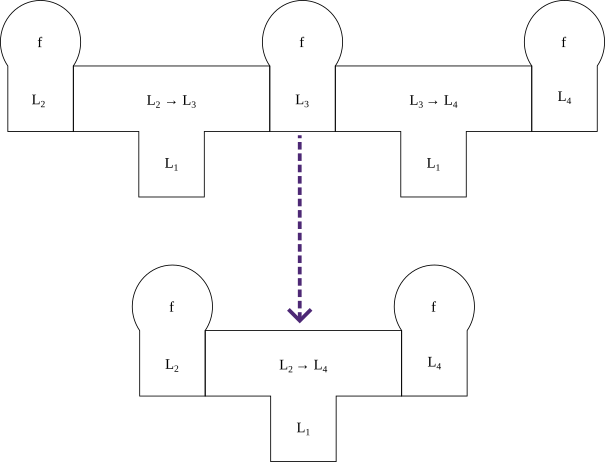
\includegraphics[width=0.66\linewidth]{./figures/summarize_compiler.png}
  \caption{Horinzontale Übersetzungszwischenschritte zusammenfassen}
  \label{fig:t_diagram_horinzontal_zusammenfassen}
\end{figure}

\begin{figure}[H]
  \centering
  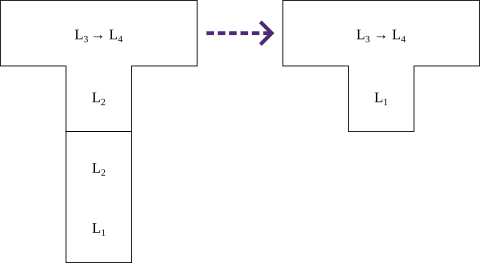
\includegraphics[width=0.5\linewidth]{./figures/summarize_interpreter.png}
  \caption{Vertikale Interpretierungszwischenschritte zusammenfassen}
  \label{fig:t_diagram_vertikal_zusammenfassen}
\end{figure}

\section{Formale Sprachen}
% EBNF erwähnen
% TODO: Was ist ein Terminalsymbol und was ist ein Nicht-Terminalsymbol
\begin{Definition}{Sprache}{Sprache}
  \footcite{nebel_theoretische_2020}
\end{Definition}
\begin{Definition}{Chromsky Hierarchie}{chromsky_hierarchie}
  \footcite{nebel_theoretische_2020}
\end{Definition}
\begin{Definition}{Grammatik}{grammatik}
  \footcite{nebel_theoretische_2020}
\end{Definition}
\begin{Definition}{Reguläre Sprachen}{reguläre_sprachen}
  \footcite{nebel_theoretische_2020}
\end{Definition}
\begin{Definition}{Kontextfreie Sprachen}{kontextfreie_sprachen}
  \footcite{nebel_theoretische_2020}
\end{Definition}
\begin{Definition}{Ableitung}{ableitung}
  \footcite{nebel_theoretische_2020}
\end{Definition}
\begin{Definition}{Links- und Rechtsableitung}{links_und_rechtsableitung}
  \footcite{nebel_theoretische_2020}
\end{Definition}
\begin{Definition}{Linksrekursive Grammatiken}{linksrekursive_grammatiken}
Eine \colorbold{Grammatik} ist \colorbold{linksrekursiv}, wenn sie ein  \colorbold{Nicht-Terminalsymbol} enthält, dass \colorbold{linksrekursiv} ist.

Ein \colorbold{Nicht-Terminalsymbol} ist  \colorbold{linksrekursiv}, wenn das \colorbold{linkeste Symbol} in einer seiner \colorbold{Produktionen} es selbst ist oder zu sich selbst gemacht werden kann durch eine Folge von Ableitungen:
\begin{equation*}
  A \Rightarrow^{*} Aa,
\end{equation*}
wobei $a$ eine beliebige Folge von \colorbold{Terminalsymbolen} und \colorbold{Nicht-Terminalsymbolen} ist.\footcite{noauthor_parsing_nodate}
\end{Definition}

\subsection{Mehrdeutige Grammatiken}
\begin{Definition}{Ableitungsbaum}{ableitungsbaum}
  \footcite{nebel_theoretische_2020}
% TODO: Bild hierfür
\end{Definition}
\begin{Definition}{Mehrdeutige Grammatik}{mehrdeutige_grammatik}
  \footcite{nebel_theoretische_2020}
% TODO: (Bild hierfür)
\end{Definition}
\subsection{Präzidenz und Assoziativität}
\begin{Definition}{Assoziativität}{assoziativität}
  \footcite{noauthor_parsing_nodate}
\end{Definition}
\begin{Definition}{Präzidenz}{präzidenz}
  \footcite{noauthor_parsing_nodate}
\end{Definition}
\begin{Definition}{Wortproblem}{wortproblem}
  \footcite{nebel_theoretische_2020}
  % zu Grammatiken schieben
\end{Definition}
\begin{Definition}{LL(k)-Grammatik}{llk_grammatik}
  Eine Grammatik ist \colorbold{LL(k)} für $k\in\mathbb{N}$, falls jeder Ableitungsschritt eindeutig durch die nächsten $k$ \colorbold{Symbole} des \colorbold{Eingabeworts} bzw. in Bezug zu Compilerbau \colorbold{Token} des \colorbold{Inputstrings} zu bestimmen ist\footnote{Das wird auch als \colorbold{Lookahead} von $k$ bezeichnet.}. Dabei steht \colorbold{LL} für \colorbold{l}eft-to-right und \colorbold{l}eftmost-derivation, da das \colorbold{Eingabewort} von \colorbold{links nach rechts} geparsed und immer \colorbold{Linksableitungen} genommen werden müssen\footnote{Wobei sich das mit den \colorbold{Linksableitungen} automatisch ergibt, wenn man das Eingabewort von  \colorbold{links-nach-rechts} parsed und jeder der nächsten $k$ \colorbold{Ableitungsschritte} eindeutig sein soll.}, damit die obige Bedingung mit den \colorbold{nächsten} $k$ Symbolen gilt.\footcite{nebel_theoretische_2020}
\end{Definition}
% \subsection{Linksrekursiv und Rechtrekursiv}
\section{Lexikalische Analyse}
\label{sec:lexikalische_analyse}

Die \colorbold{Lexikalische Analyse} bildet üblicherweise die erste Ebene innerhalb des \colorbold{Pipe-Filter Architekturpatterns} (Definition~\ref{def:pipe_architektur}) bei der Implementierung von Compilern. Die Aufgabe der lexikalischen Analyse ist vereinfacht gesagt, in einem Inputstring, z.B. dem Inhalt einer Datei, welche in \colorbold{UTF-8} codiert ist, Folgen endlicher Symbole (auch \colorbold{Wörter} genannt) zu finden, die bestimmte \colorbold{Pattern} (Definition~\ref{def:pattern}) matchen, die durch eine \colorbold{reguläre Grammatik} spezifiziert sind.

\begin{Definition}{Pipe-Filter Architekturpattern}{pipe_architektur}
  Ist ein \colorbold{Archikteturpattern}, welches aus \colorbold{Pipes} und \colorbold{Filtern} besteht, wobei der \colorbold{Ausgang} eines \colorbold{Filters} der \colorbold{Eingang} des durch eine \colorbold{Pipe} verbundenen adjazenten nächsten \colorbold{Filters} ist, falls es einen gibt.

  Ein \colorbold{Filter} stellt einen Schritt dar, indem eine Eingabe \colorbold{weiterverarbeitet} wird und \colorbold{weitergereicht} wird. Bei der \colorbold{Weiterverarbeitung} können Teile der Eingabe \colorbold{entfernt}, \colorbold{hinzugefügt} oder \colorbold{vollständig ersetzt} werden.

  Eine \colorbold{Pipe} stellt ein \colorbold{Bindeglied} zwischen zwei \colorbold{Filtern} dar.\footnote{Das ein \colorbold{Bindeglied} eine eigene Bezeichnung erhält, bedeutet allerdings nicht, dass es eine eigene wichtige \colorbold{Aufgabe} erfüllt. Wie bei vielen \colorbold{Pattern}, soll mit dem Namen des \colorbold{Pattern}, in diesem Fall durch das \colorbold{Pipe} die Anlehung an z.B. die \colorbold{Pipes aus Unix}, z.B. \smalltt{cat /proc/bus/input/devices | less} zum Ausdruck gebracht werden. Und so banal es klingt, sollen manche Bezeichnungen von Pattern auch einfach nur gut klingen.}\footcite{westphal_softwaretechnik_2021}

  \begin{figure}[H]
    \centering
    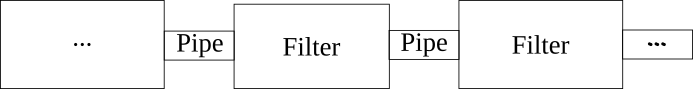
\includegraphics[width=0.66\linewidth]{./figures/pipe_architecture.png}
  \end{figure}
\end{Definition}

Diese Folgen endlicher Symoble werden auch \colorbold{Lexeme} (Definition~\ref{def:lexeme}) genannt.

\begin{Definition}{Pattern}{pattern}
  \colorbold{Beschreibung} aller möglichen \colorbold{Lexeme}, die eine Menge $\mathbb{P}_{T}$ bilden und einem bestimmten \colorbold{Token} $T$ zugeordnet werden.
  Die Menge $\mathbb{P}_{T}$ ist eine möglicherweise unendliche Menge von \colorbold{Wörtern}, die sich mit den Produktionen einer \colorbold{regulären Grammatik} ${G}_{Lex}$ einer \colorbold{regulären Sprache} ${L}_{Lex}$ beschreiben lassen \footnote{Als Beschreibungswerkzeug können aber auch z.B. reguläre Ausdrücke hergenommen werden.}, die für die Beschreibung eines \colorbold{Tokens} $T$ zuständig sind.\footcite{thiemann_compilerbau_2021}
\end{Definition}

\begin{Definition}{Lexeme}{lexeme}
  Ein \colorbold{Lexeme} ist ein \colorbold{Wort} aus dem Inputstring, welches das \colorbold{Pattern} für eines der \colorbold{Token} $T$ einer \colorbold{Sprache} ${L}_{Lex}$ matched.\footcite{thiemann_compilerbau_2021}
\end{Definition}

Diese \colorbold{Lexeme} werden vom \colorbold{Lexer} (Definition~\ref{def:lexer}) im \colorbold{Inputstring} identifziert und \colorbold{Tokens} $T$ zugeordnet. Das jeweils nächste \colorbold{Lexeme} fängt dabei genau nach dem letzten Symbol des \colorbold{Lexemes} an, das zuletzt vom \colorbold{Lexer} erkannt wurde. Die \colorbold{Tokens} (Definition~\ref{def:lexer}) sind es, die letztendlich an die \colorbold{Syntaktische Analyse} weitergegeben werden.

\begin{Definition}{Lexer (bzw. Scanner oder auch Tokenizer)}{lexer}
  Ein \colorbold{Lexer} ist eine \colorbold{partielle} Funktion \hspace{0.2cm}$lex: \Sigma^{*} \rightharpoonup (N \times W)^{*}$, welche ein \colorbold{Wort} bzw. \colorbold{Lexeme} aus $\Sigma^{*}$ auf ein \colorbold{Token} $T$ mit einem \colorbold{Tokennamen} $N$ und einem \colorbold{Tokenwert} $W$ abbildet, falls dieses \colorbold{Wort} sich unter der \colorbold{regulären Grammatik} ${G}_{Lex}$, der \colorbold{regulären Sprache} ${L_{Lex}}$ abbleiten lässt bzw. einem der \colorbold{Pattern} der Sprache $L_{Lex}$ entspricht.\footcite{thiemann_compilerbau_2021}
\end{Definition}

Ein \colorbold{Lexer} ist im Allgemeinen eine \colorbold{partielle Funktion}, da es Zeichenfolgen geben kann, die kein \colorbold{Pattern} eines \colorbold{Tokens} der Sprache $L_{Lex}$ matchen. In Bezug auf eine Implementierung, wird, wenn der Lexer Teil der Implementierung eines Compilers ist, in diesem Fall eine \colorbold{Fehlermeldung} ausgegeben.

\begin{Special_Paragraph}
  Um Verwirrung verzubäugen ist es wichtig folgende Unterscheidung hervorzuheben:

  Wenn von \colorbold{Symbolen} die Rede ist, so werden in der \colorbold{Lexikalischen Analyse}, der \colorbold{Syntaktische Analyse} und der \colorbold{Code Generierung}, auf diesen verschiedenen Ebenen unterschiedliche Konzepte als Symbole bezeichnet.

  In der Lexikalischen Analyse sind einzelne \colorbold{Zeichen eines Zeichensatzes} die Symbole.

  In der Syntaktischen Analyse sind die \colorbold{Tokennamen} die Symbole.

  In der Code Generierung sind die \colorbold{Bezeichner} (Definition~\ref{def:bezeichner}) von \colorbold{Variablen, Konstanten und Funktionen} die Symbole\footnote{Das ist der Grund, warum die \colorbold{Tabelle}, in der Informationen zu \colorbold{Bezeichnern} gespeichert werden, in Kapitel~\ref{ch:implementierung} \colorbold{Symboltabelle} genannt wird.}.
\end{Special_Paragraph}

\begin{Definition}{Bezeichner (bzw. Identifier)}{bezeichner}
  \colorbold{Tokenwert}, der eine Konstante, Variable, Funktion usw. innerhalb ihres \colorbold{Scopes} \colorbold{eindeutig} benennt.\footnote{Außer wenn z.B. bei Funktionen die Programmiersprache das \colorbold{Überladen} erlaubt usw. In diesem Fall wird die \colorbold{Signatur} der Funktion als weiteres Unterschiedungsmerkmal hinzugenommen, damit es eindeutig ist.}\footcite{thiemann_einfuhrung_2018}
\end{Definition}

Eine weitere Aufgabe der \colorbold{Lekikalischen Analyse} ist es jegliche für die Weiterverarbeitung unwichtigen Symbole, wie Leerzeichen \,\textvisiblespace\,, Newline \verb|\n|\footnote{In Unix Systemen wird für Newline das ASCII Symbol \colorbold{line feed}, in Windows hingegen die ASCII Symbole \colorbold{carriage return} und \colorbold{line feed} nacheinander verwendet. Das wird aber meist durch die verwendete Porgrammiersprache, die man zur Inplementierung des Lexers nutzt wegabstrahiert.} und Tabs \verb|\t| aus dem Inputstring herauszufiltern. Das geschieht mittels des \colorbold{Lexers}, der allen für die \colorbold{Syntaktische Analyse} unwichtige Zeichen das leere Wort $\epsilon$ zuordnet. Das ist auch im Sinne der Definition, denn $\epsilon \in (N\times W)^{*}$ ist immer der Fall beim \colorbold{Kleene Stern Operator} $^{*}$. Nur das, was für die \colorbold{Syntaktische Analyse} wichtig ist, soll weiterverarbeitet werden, alles andere wird herausgefiltert.

Der Grund warum nicht einfach nur die \colorbold{Lexeme} an die \colorbold{Syntaktische Analyse} weitergegeben werden und der Grund für die Aufteilung des \colorbold{Tokens} in \colorbold{Tokenname} und \colorbold{Tokenwert} ist, weil z.B. die Bezeichner von Variablen, Konstanten und Funktionen beliebige Zeichenfolgen sein können, wie \smalltt{my\_fun}, \smalltt{my\_var} oder \smalltt{my\_const} und es auch viele verschiedenen Zahlen gibt, wie \smalltt{42}, \smalltt{314} oder \smalltt{12}. Die \colorbold{Überbegriffe} bzw. \colorbold{Tokennamen} für beliebige Bezeichner von Variablen, Konstanten und Funktionen und beliebige Zahlen sind aber trotz allem z.B. \smalltt{NAME} und \smalltt{NUM}\footnote{Diese \colorbold{Tokennamen} wurden im  \colorbold{PicoC-Compiler} verwendet, da man beim Programmieren möglichst \colorbold{kurze} und \colorbold{leicht verständliche} Bezeichner für seine Nodes haben will, damit unter anderem \colorbold{mehr Code} in eine Zeile passt.}, bzw. wenn man sich nicht Kurzformen sucht \smalltt{IDENTIFIER} und \smalltt{NUMBER}. Für \colorbold{Lexeme}, wie \verb|if| oder \verb|}| sind die \colorbold{Tokennamen} bzw. Überbegriffe genau die Bezeichnungen, die man diesen Zeichenfolgen geben würde, nämlich \smalltt{IF} und \smalltt{RBRACE}.

Ein \colorbold{Lexeme} ist damit aber nicht immer das gleiche, wie der \colorbold{Tokenwert}, denn z.B. im Falle von PicoC kann der Wert $99$ durch zwei verschiedene \colorbold{Literale} (Definition~\ref{def:literal}) dargestellt werden, einmal als ASCII-Zeichen \smalltt{'c'}, dass den entsprechenden Wert in der ASCII-Tabelle hat und des Weiteren auch in Dezimalschreibweise als \smalltt{99}\footnote{Die Programmiersprache \colorbold{Python} erlaubt es z.B. dieser Wert auch mit den Literalen \smalltt{0b1100011} und \smalltt{0x63} darzustellen.}. Der \colorbold{Tokenwert} ist jedoch der letztendlich verwendete Wert an sich, unabhängig von der Darstellungsform.

Die \colorbold{Grammatik} $G_{Lex}$, die zur Beschreibung der Token $T$ der Sprache $L_{Lex}$ verwendet wird ist üblicherweise \colorbold{regulär}, da ein typischer \colorbold{Lexer} immer nur \colorbold{ein Symbol} vorausschaut\footnote{Man nennt das auch einem \colorbold{Lookahead} von $1$}, sich nichts merken muss und unabhängig davon, was für Symbole davor aufgetaucht sind läuft. Die Grammatik~\ref{gr:concrete_syntax_lex_teil_1} liefert den Beweis, dass die Sprache $L_{PicoC\_Lex}$ des \colorbold{PicoC-Compilers} auf jeden Fall \colorbold{regulär} ist, da sie fast die Definition~\ref{def:reguläre_sprachen} erfüllt. Einzig die Produktion \verb|CHAR ::= "'"ASCII_CHAR"'"| sieht problematisch aus, kann allerdings auch als \verb|{CHAR ::= "'"CHAR2, CHAR2 ::= ASCII_CHAR"'"}| \colorbold{regulär} ausgedrückt werden\footnote{Eine derartige Regel würde nur Probleme bereiten, wenn sich aus \smalltt{ASCII\_CHAR} \colorbold{beliebig breite} Wörter ableiten liesen.}. Somit existiert eine \colorbold{reguläre Grammatik}, welche die \colorbold{Sprache} $L_{PicoC\_Lex}$ beschreibt und damit ist die \colorbold{Sprache} $L_{PicoC\_Lex}$ \colorbold{regulär}.

\begin{Definition}{Literal}{literal}
  Eine von möglicherweise vielen weiteren \colorbold{Darstellungsformen} (als \colorbold{Zeichenkette}) für ein und denselben \colorbold{Wert} eines \colorbold{Datentyps}.\footcite{thiemann_einfuhrung_2018}
  \begin{figure}[H]
    \centering
    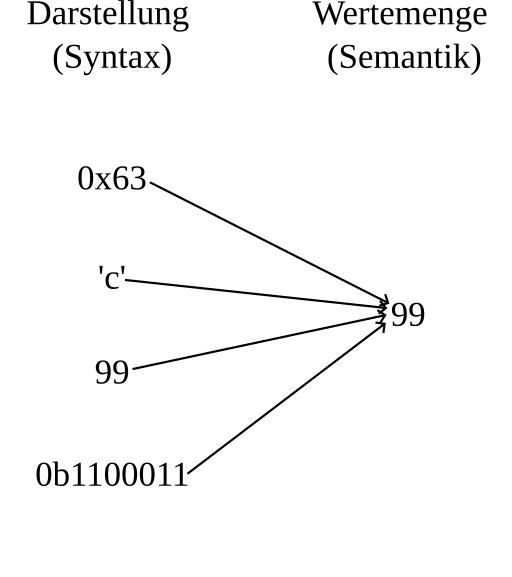
\includegraphics[width=0.33\linewidth]{./figures/literal.png}
  \end{figure}
\end{Definition}

Um eine Gesamtübersicht über die \colorbold{Lexikalische Analyse} zu geben, ist in Abbildung~\ref{fig:lexikalische_analyse_veranschaulichung} die Lexikalische Analyse an einem Beispiel veranschaulicht.

\begin{figure}[H]
  \codebox[title=Inputstring, remember as=inputstring, hbox, nobeforeafter, minted language=c]{./code_examples/example1.picoc}
  \hfill
  \codebox[title=Tokenfolge, remember as=tokenfolge, width=0.6\linewidth, nobeforeafter, minted language=text]{./code_examples/example1.tokens}

  \begin{tikzpicture}[overlay,remember picture,line width=1mm,draw=PrimaryColor]
  \draw[->] (inputstring.east) to[bend right] node[above] {Lexer} (tokenfolge.west);
  \end{tikzpicture}
  \caption{Veranschaulichung der Lexikalischen Analyse}
  \label{fig:lexikalische_analyse_veranschaulichung}
\end{figure}

\section{Syntaktische Analyse}
In der \colorbold{Syntaktischen Analyse} ist für einige Sprachen eine \colorbold{Kontextfreie Grammatik} $G_{Parse}$ notwendig, um diese Sprachen zu beschreiben, da viele Programmiersprachen z.B. für \colorbold{Funktionsaufrufe} \verb|fun(arg)| und \colorbold{Codeblöcke} \verb|if(1){}| syntaktische Mittel verwenden, die es notwendig machen sich zu merken, wieviele öffnende runde Klammern \verb|'('| bzw. öffnende geschweifte Klammern \verb|'{'| es momentan gibt, die noch nicht durch eine entsprechende schließende runde Klammer \verb|')'| bzw. schließende geschweifte Klammer \verb|'}'| geschlossen wurden.

% TODO: später erwähnen, dass alle Produktionen der Grammatik G_parse eine kontexfreie Form haben, was der Beweis ist

Die \colorbold{Syntax}, in welcher der \colorbold{Inputstring} aufgeschrieben ist, wird auch als \colorbold{Konkrette Syntax} (Definition~\ref{def:konkrette_syntax}) bezeichnet. In einem Zwischenschritt, dem \colorbold{Parsen} wird aus diesem Inputstring mithilfe eines \colorbold{Parsers} (Definition~\ref{def:parser}), ein \colorbold{Derivation Tree} (Definition~\ref{def:derivation_tree}) generiert, der als Zwischenstufe hin zum einem \colorbold{Abstract Syntax Tree} (Definition~\ref{def:abstrakte_syntax_tree}) dient. Beim Compilerbau ist es förderlich kleinschrittig vorzugehen, deshalb erst die Generierung des \colorbold{Derivation Tree} und dann erst des \colorbold{Abstract Syntax Tree}.

\begin{Definition}{Konkrette Syntax}{konkrette_syntax}
  \colorbold{Syntax} einer \colorbold{Sprache}, die durch die \colorbold{Grammatiken} $G_{Lex}$ und $G_{Parse}$ zusammengenommen beschrieben wird.

  Ein \colorbold{Programm} in seiner \colorbold{Textrepräsentation}, wie es in einer Textdatei nach den Produktionen der \colorbold{Grammatiken} $G_{Lex}$ und $G_{Parse}$ abgeleitet steht, bevor man es kompiliert, ist in \colorbold{Konkretter Syntax} aufgeschrieben.\footcite{g_siek_course_2022}
\end{Definition}

\begin{Definition}{Derivation Tree (bzw. Parse Tree)}{derivation_tree}
  \colorbold{Compilerinterne Darstellung} eines in \colorbold{Konkretter Syntax} geschriebenen Inputstrings als \colorbold{Baumdatenstruktur}, in der \colorbold{Nichtterminalsymbole} die \colorbold{Inneren Knoten} der Baumdatenstruktur und \colorbold{Terminalsymbole} die \colorbold{Blätter} der Baumdatenstruktur bilden. Jedes zum Ableiten des Inputstrings verwendetete \colorbold{Nicht-Terminalsymbol} einer \colorbold{Produktion} der \colorbold{Grammatik} $G_{Parse}$, die ein Teil der \colorbold{Konkrette Syntax} ist,  bildet einen eigenen \colorbold{Inneren Knoten}.

  Der \colorbold{Derivation Tree} wird optimalerweise immer so konstruiert bzw. die \colorbold{Konkrette Syntax} immer so definiert, dass sich möglichst einfach ein \colorbold{Abstract Syntax Tree} daraus konstruieren lässt.\footcite{noauthor_json_nodate}
% TODO: vielleicht ein hübsches Bildchen
\end{Definition}

\begin{Definition}{Parser}{parser}
  Ein \colorbold{Parser} ist ein Programm, dass aus einem Inputstring, der in \colorbold{Konkretter Syntax} geschrieben ist, eine compilerinterne Darstellung, den \colorbold{Derivation Tree} generiert, was auch als  \colorbold{Parsen} bezeichnet wird\footnote{Es gibt allerdings auch alternative Definitionen, denen nach ein Parser in Bezug auf Compilerbau ein Programm ist, dass einen Inputstring von \colorbold{Konkretter Syntax} in  \colorbold{Abstrakte Syntax} übersetzt. Im Folgenden wird allerdings die Definition \ref{def:parser} verwendet.}.\footcite{noauthor_json_nodate}
\end{Definition}

\begin{Special_Paragraph}
  An dieser Stelle könnte möglicherweise eine Verwirrung enstehen, welche Rolle dann überhaupt ein \colorbold{Lexer} hier spielt.

  In Bezug auf Compilerbau ist ein \colorbold{Lexer} ein Teil eines \colorbold{Parsers}. Der \colorbold{Lexer} ist auschließlich für die \colorbold{Lexikalische Analyse} verantwortlich und entspricht z.B., wenn man bei einem Wanderausflug verschiedenen Insekten entdeckt, dem Nachschlagen in einem Insekten\colorbold{lexikon} und dem Aufschreiben, welchen Insekten man in welcher \colorbold{Reihenfolge} begegnet ist. Zudem kann man bestimmte \colorbold{Sehenswürdigkeiten} an denen man während des Ausflugs vorbeikommt ebenfalls festhalten, da es eine Rolle spielen kann in welchem örtlichen \colorbold{Kontext} man den Insekten begegnet ist\footnote{Das würde z.B. der Rolle eines \colorbold{Semikolon} \smalltt{;} in der Sprache $L_{PicoC}$ entsprechen.}.

  Der \colorbold{Parser} vereinigt sowohl die \colorbold{Lexikalische Analyse}, als auch einen Teil der \colorbold{Syntaktischen Analyse} in sich und entspricht, um auf das Beispiel zurückzukommen, dem Darstellen von \colorbold{Beziehungen} zwischen den Insektenbegnungen in einer für die \colorbold{Weiterverarbeitung tauglichen Form}\footnote{Z.B. gibt es bestimmte \colorbold{Wechselbeziehungen} zwischen Insekten, Insekten beinflussen sich gegenseitig.}.

  In der Weiterverarbeitung kann der \colorbold{Interpreter} das interpretieren und daraus bestimmte Schlüsse ziehen und ein  \colorbold{Compiler} könnte es vielleicht in eine für Menschen leichter entschüsselbare Sprache kompilieren.
\end{Special_Paragraph}

Die vom \colorbold{Lexer} im Inputstring identifizierten \colorbold{Token} werden in der \colorbold{Syntaktischen Analyse} vom \colorbold{Parser} als \colorbold{Wegweiser} verwendet, da je nachdem, in welcher Reihenfolge die \colorbold{Token} auftauchen, dies einer anderen Ableitung in der \colorbold{Grammatik} $G_{Parse}$ entspricht. Dabei wird in der Grammatik $L_{Parse}$ nach dem \colorbold{Tokennamen} unterschieden und nicht nach dem Tokenwert, da es nur von Interesse ist, ob an einer bestimmten Stelle z.B. eine \verb|Zahl| steht und nicht, welchen konkretten Wert diese \verb|Zahl| hat. Der \colorbold{Tokenwert} ist erst später in der \colorbold{Code Generierung} in~\ref{sec:code_generierung} wieder relevant.

Ein \colorbold{Parser} ist genauergesagt ein erweiterter \colorbold{Recognizer} (Definition~\ref{def:recognizer}), denn ein Parser löst das \colorbold{Wortproblem} (Definition~\ref{def:wortproblem}) für die \colorbold{Sprache}, die durch die \colorbold{Konkrette Syntax} beschrieben wird und konstruiert parallel dazu oder im Nachgang aus den Informationen, die während der Ausführung des Recognition Algorithmus gesichert wurden den \colorbold{Derivation Tree}.

\begin{Definition}{Recognizer (bzw. Erkenner)}{recognizer}
  Entspricht dem Maschienenmodell eines \colorbold{Automaten}. Im Bezug auf Compilerbau entspricht der \colorbold{Recognizer} einem \colorbold{Kellerautomaten}, in dem \colorbold{Wörter} bestimmter \colorbold{Kontextfreier Sprachen} erkannt werden. Der \colorbold{Recognizer} erkennt, ob ein Inputstring bzw. \colorbold{Wort} sich mit den Produktionen der \colorbold{Konkrette Syntax} ableiten lässt, also ob er bzw. es Teil der Sprache ist, die von der \colorbold{Konkretten Syntax} beschrieben wird oder nicht\footnote{Das vom \colorbold{Recognizer} gelöste Problem ist auch als \colorbold{Wortproblem} bekannt.}\footcite{thiemann_compilerbau_2021}
\end{Definition}

\begin{Special_Paragraph}
Für das \colorbold{Parsen} gibt es grundsätzlich \colorbold{zwei} verschiedene Ansätze:

% https://tex.stackexchange.com/questions/12373/how-to-change-the-space-between-the-itemize-items-in-latex
% https://stackoverflow.com/questions/1061112/eliminate-space-before-beginitemize
\begin{itemize}[itemsep=-1mm, topsep=-1mm]
  \coloritem[Top-Down Parsing] Der \colorbold{Derivation Tree} wird von \colorbold{oben-nach-unten} generiert, also von der \colorbold{Wurzel} zu den \colorbold{Blättern}. Dementsprechend fängt die Generierung des \colorbold{Derivation Tree} mit dem \colorbold{Startsymbol} der \colorbold{Grammatik} an und wendet in jedem Schritt eine \colorbold{Linksableitung} auf die \colorbold{Nicht-Terminalsymbole} an, bis man \colorbold{Terminalsymbole} hat, die sich zum gewünschten \colorbold{Inputstring} abgeleitet haben oder sich herausstellt, dass dieser nicht abgeleitet werden kann.\footcite{noauthor_what_nodate-2}

  Der Grund, warum die \colorbold{Linksableitung} verwendet wird und nicht z.B. die \colorbold{Rechtsableitung}, ist, weil der \colorbold{Eingabewert} bzw. der \colorbold{Inputstring} von \colorbold{links nach rechts} eingelesen wird, was gut damit zusammenpasst, dass die \colorbold{Linksableitung} die \colorbold{Blätter} von \colorbold{links-nach-rechts} generiert.

  Welche der \colorbold{Produktionen} für ein \colorbold{Nicht-Terminalsymbol} angewandt wird, wenn es mehrere \colorbold{Alternativen} gibt, wird entweder durch \colorbold{Backtracking} oder durch \colorbold{Vorausschauen} gelöst.

  Eine sehr einfach zu implementierende Technik für \colorbold{Top-Down Parser} ist hierbei der \colorbold{Rekursive Abstieg}. Dabei wird jedem \colorbold{Nicht-Terminalsymbol} eine \colorbold{Prozedur} zugeordnet, welche die \colorbold{Produktionen} dieses Nicht-Terminalsymbols umsetzt. \colorbold{Prozeduren} rufen sich dabei wechselseitig gegenseitig entsprechend der Produktionsregeln auf, falls eine Produktionsregel ein entsprechendes \colorbold{Nicht-Terminal} enthält.

  Mit dieser Methode ist das Parsen \colorbold{Linksrekursiver Grammatiken} (Definition~\ref{def:linksrekursive_grammatiken}) allerdings nicht möglich, ohne die Grammatik vorher umgeformt zu haben und jegliche \colorbold{Linksrekursion} aus der \colorbold{Grammatik} entfernt zu haben, da diese zu \colorbold{Unendlicher Rekursion} führt.

  \colorbold{Rekursiver Abstieg} kann mit \colorbold{Backtracking} verbunden werden, um auch Grammatiken parsen zu können, die nicht \colorbold{LL(k)} (Definition~\ref{def:llk_grammatik}) sind. Dabei werden meist nach dem \colorbold{Depth-First-Search Prinzip} alle \colorbold{Produktionen} für ein \colorbold{Nicht-Terminalsymbol} solange durchgegangen bis der gewüschte Inpustring abgeleitet ist oder alle \colorbold{Alternativen} für einen Schritt abgesucht sind, bis man wieder beim ersten Schritt angekommen ist und da auch alle \colorbold{Alternativen} abgesucht sind, was dann bedeutet, dass der \colorbold{Inputstring} sich \colorbold{nicht} mit der verwendeten Grammatik ableiten lässt.\footnote{Diese Form von Parsing wurde im \colorbold{PicoC-Compiler} implementiert, als dieser noch auf dem Stand des \colorbold{Bachelorprojektes} war, bevor er durch den nicht selbst implementierten \colorbold{Earley Parser} von \colorbold{Lark} (siehe \cite{noauthor_lark_2022}) ersetzt wurde.}

  Wenn man eine \colorbold{LL(k)} Grammatik hat, kann man auf \colorbold{Backtracking verzichten} und es reicht einfach nur immer $k$  \colorbold{Token} im Inputstring \colorbold{vorauszuschauen}. \colorbold{Mehrdeutige Grammatiken} sind dadurch ausgeschlossen, weil \colorbold{LL(k)} keine \colorbold{Mehrdeutigkeit} zulässt.\footnote{Diese Art von Parser ist im \colorbold{RETI-Interpreter} implementiert, da die \colorbold{RETI-Sprache} eine besonders simple \colorbold{LL(1) Grammatik} besitzt. Diese Art von \colorbold{Parser} wird auch als \colorbold{Predictive Parser} oder \colorbold{LL(k) Recursive Descent Parser} bezeichnet, wobei \colorbold{Recursive Descent} das englische Wort für \colorbold{Rekursiven Abstieg} ist.}
  \coloritem[Bottom-Up Parsing] Es wird mit dem \colorbold{Eingabewort} bzw. \colorbold{Inputstring} gestartet und versucht \colorbold{Rechtsableitungen} entsprechend der \colorbold{Produktionen} der \colorbold{Konkretten Syntax} rückwärts anzuwenden, bis man beim \colorbold{Startsymbol} landet.\footcite{noauthor_what_nodate-1}
  \coloritem[Chart Parser] Es wird \colorbold{Dynamische Programmierung} verwendet und partielle Zwischenergebnisse werden in einer \colorbold{Tabelle} (bzw. einem \colorbold{Chart}) gespeichert und können wiederverwendet werden. Das macht das Parsen \colorbold{Kontextfreier Grammatiken} effizienter, sodass es nur noch \colorbold{polynomielle} Zeit braucht, da \colorbold{Backtracking} nicht mehr notwendig ist.\footnote{Der \colorbold{Earley Parser}, den \colorbold{Lark} und damit der \colorbold{PicoC-Compiler} verwendet fällt unter diese Kategorie.}
  % TODO: nachdenken das polynomiel zu streichen
\end{itemize}
  % ein hübsches Bildchen, wo man einen Überblick bekommt
\end{Special_Paragraph}

% Problem mit Linksrekursion und Mehrdeutigkeit ansprechen

Der \colorbold{Abstract Syntax Tree} wird mithilfe von \colorbold{Transformern} (Definition~\ref{def:transformer}) und \colorbold{Visitors} (Definition~\ref{def:visitor}) generiert und ist das Endprodukt der \colorbold{Syntaktischen Analyse}, welches an die \colorbold{Code Generierung} weitergegeben wird. Wenn man die gesamte \colorbold{Syntaktische Analyse} betrachtet, so übersetzt diese einen Inputstring von der \colorbold{Konkretten Syntax} in die \colorbold{Abstrakte Syntax} (Definition~\ref{def:abstrakte_syntax}).

\begin{Definition}{Transformer}{transformer}
  Ein Programm, dass von \colorbold{unten-nach-oben}, nach dem \colorbold{Breadth First Search} Prinzip alle Knoten des \colorbold{Derivation Tree} besucht und beim Antreffen eines bestimmten Knoten des \colorbold{Derivation Tree} einen entsprechenden Knoten des \colorbold{Abstract Syntax Tree} erzeugt und diesen anstelle des Knotens des \colorbold{Derivation Tree} setzt und so Stück für Stück den \colorbold{Abstract Syntax Tree} konstruiert.\footcite{noauthor_transformers_nodate}
\end{Definition}

\begin{Definition}{Visitor}{visitor}
  Ein Programm, dass von \colorbold{unten-nach-oben}, nach dem \colorbold{Breadth First Search} Prinzip alle Knoten des \colorbold{Derivation Tree} besucht und in Bezug zu Compilerbau, beim Antreffen eines bestimmten \colorbold{Knoten} des Derivation Tree, diesen \colorbold{in-place} mit anderen Knoten \colorbold{tauscht} oder \colorbold{manipuliert}, um den Derivation Tree für die weitere Verarbeitung durch z.B. einen Transformer zu vereinfachen.\footnote{Kann theoretisch auch zur Konstruktion eines \colorbold{Abstract Syntax Tree} verwendet werden, wenn z.B. eine externe Klasse verwendet wird, welches für die Konstruktion des \colorbold{Abstract Syntax Tree} verantwortlich ist. Aber dafür ist ein \colorbold{Transformer} besser geeignet.}\footcite{noauthor_transformers_nodate}
\end{Definition}

\begin{Definition}{Abstrakte Syntax}{abstrakte_syntax}
  \colorbold{Syntax}, die beschreibt, was für Arten von \colorbold{Komposition} bei den \colorbold{Knoten} eines \colorbold{Abstract Syntax Trees} möglich sind.

  Jene Produktionen, die in der \colorbold{Konkretten Syntax} für die Umsetzung von \colorbold{Präzidenz} notwendig waren, sind in der \colorbold{Abstrakten Syntax} abgeflacht.\footcite{g_siek_course_2022}
\end{Definition}

\begin{Definition}{Abstract Syntax Tree (AST)}{abstrakte_syntax_tree}
  \colorbold{Compilerinterne Darstellung} eines Programs, in welcher sich anhand der Knoten auf dem \colorbold{Pfad} von der \colorbold{Wurzel} zu einem \colorbold{Blatt} nicht mehr direkt nachvollziehen lässt, durch welche \colorbold{Produktionen} dieses Blatt abgeleitet wurde.

Der \colorbold{Abstract Syntax Tree} hat einmal den Zweck, dass die \colorbold{Kompositionen}, die die Knoten bilden können \colorbold{semantisch} näher an den \colorbold{Instructions eines Assemblers} dran sind und, dass man mit einem \colorbold{Abstract Syntax Tree} bei der Betrachtung eines \colorbold{Knoten}, der für einen Teil des Programms steht, möglichst schnell die Fragen beantworten kann, welche \colorbold{Funktionalität} der Sprache dieser umsetzt, welche \colorbold{Bestandteile} er hat und welche \colorbold{Funktionalität} der Sprache diese Bestandteile umsetzen usw.\footcite{g_siek_course_2022}
\end{Definition}

Die \colorbold{Baumdatenstruktur} des \colorbold{Derivation Tree} und \colorbold{Abstract Syntax Tree} ermöglicht es die Operationen, die ein Compiler bzw. Interpreter bei der Weiterverarbeitung des Inputstrings ausführen muss möglichst \colorbold{effizient} auszuführen und auf \colorbold{unkomplizierte} Weise direkt zu erkennen, welche er ausführen muss.

% Je weiter \colorbold{unten}\footnote{In der Informatik wachsen \colorbold{Bäume} von \colorbold{oben-nach-unten}. Die \colorbold{Wurzel} ist also \colorbold{oben}.} und \colorbold{links} ein Knoten im \colorbold{Abstract Syntax Tree} liegt, desto eher wird dieser Knoten komplett abgearbeitet sein, da in der \colorbold{Code Generierung} die Knoten nach dem \colorbold{Depth First Search} Prinzip abgearbeitet werden.
% nur bei Top-Down!

Um eine Gesamtübersicht über die \colorbold{Syntaktische Analyse} zu geben, ist in Abbildung~\ref{fig:syntaktische_analyse_veranschaulichung} die Syntaktische mit dem Beispiel aus Subkapitel~\ref{sec:lexikalische_analyse} fortgeführt.

\pagebreak
% https://tex.stackexchange.com/questions/8625/force-figure-placement-in-text
\begin{figure}[H]
  \centering
  \codebox[title=Tokenfolge, remember as=tokenfolge, width=0.6\linewidth, nobeforeafter, minted language=text]{./code_examples/example1.tokens}
  \hfill
  \codebox[title=Abstract Syntax Tree, remember as=abstract_sytax_tree, hbox, nobeforeafter, minted language=text]{./code_examples/example1.ast}
  \vspace{2cm}
  \codebox[title=Derivation Tree, remember as=derivation_tree, hbox, minted language=text]{./code_examples/example1.dt}

  \begin{tikzpicture}[overlay,remember picture,line width=1mm,draw=PrimaryColor]
    \draw[->] (tokenfolge.south) to node[left] {Parser} (derivation_tree.north);
    \draw[->] (derivation_tree.north) to node[right] {Visitors und Transformer} (abstract_sytax_tree.south);
  \end{tikzpicture}
  \caption{Veranschaulichung der Syntaktischen Analyse}
  \label{fig:syntaktische_analyse_veranschaulichung}
\end{figure}
% TODO: extra untersciedliche Darstellungsweise gewählt für DT und AST

\section{Code Generierung}
\label{sec:code_generierung}

In der \colorbold{Code Generierung} steht man nun dem Problem gegenüber einen \colorbold{Abstract Syntax Tree} einer Sprache $L_1$ in den \colorbold{Abstract Syntax Tree} einer Sprache $L_2$ umformen zu müssen. Dieses Problem lässt sich vereinfachen, indem man das Problem in mehrere Schritte unterteilt, die man \colorbold{Passes} (Definition~\ref{def:pass}) nennt.

\begin{Special_Paragraph}
  Man spricht hier von dem \colorbold{\dq Abstrakt Syntax Tree einer Sprache $L_{1}$ (bzw. $L_{2}$)\dq} und meint damit eine \colorbold{Sprache}, die durch eine \colorbold{Konkrette Syntax} beschrieben wird und nicht durch die \colorbold{Abstrakte Syntax}, nach welcher der \colorbold{Abstract Syntax Tree} abgeleitet ist. Hierbei handelt es sich um eine im Compilerbau geläufige \colorbold{Redeart}, die vielleicht verwirrend sein kann. Man will mit der \colorbold{ersteren Redeart} ausdrücken, dass der \colorbold{Abstrakt Syntax Tree} der zur Sprache $L_{1}$ (bzw. $L_2$) passend kontruierte \colorbold{Abstract Syntax Tree} ist. Für die tatsächliche Sprache, die durch die \colorbold{Abstrakt Syntax} beschrieben wird, interessiert man sich nicht explizit. Diese \colorbold{Redeart} wurde aus der \colorbold{Quelle} \cite{g_siek_course_2022} übernommen.
\end{Special_Paragraph}

\begin{Definition}{Pass}{pass}
  \colorbold{Einzelner Übersetzungsschritt} in einem \colorbold{Kompiliervorgang} von einem \colorbold{Abstract Syntax Tree} $A_i$ einer Sprache $L_i$ zu einem \colorbold{Abstract Syntax Tree} $A_{i+1}$ einer Sprache $L_{i+1}$, der meist \colorbold{eine} bestimmte \colorbold{Teilaufgabe} übernimmt, die sich mit keiner \colorbold{Teilaufgabe} eines anderen \colorbold{Passes} überschneidet und möglichst wenig \colorbold{Ähnlichkeit} mit den \colorbold{Teilaufgaben} anderer \colorbold{Passes} haben sollte.\footnote{$L_i$ bzw. $L_{i+1}$ sind hierbei keine \colorbold{Sprachen}, die durch eine \colorbold{Abstrakte Syntax} beschrieben werden, sondern Sprachen, die durch eine \colorbold{Konkrette Syntax} beschrieben werden.}\footnote{Ein \colorbold{Pass} kann mit einem \colorbold{Transpiler}~\ref{def:transpiler} (Definition~\ref{def:transpiler}) verglichen werden, da sich die zwei Sprachen $L_i$ und  $L_{i+1}$ aufgrund der \colorbold{Kleinschrittigkeit} meist auf einem ähnlichen \colorbold{Abstraktionslevel} befinden. Der Unterschied ist allerdings, dass ein \colorbold{Transpiler} zwei Programme, die in $L_i$ bzw.  $L_{i+1}$ geschrieben sind kompiliert. Ein \colorbold{Pass} ist dagegen immer \colorbold{kleinschrittig} und operiert auf \colorbold{Abstract Syntax Trees}.}

  % man tut so als gäbe es

  Für jeden \colorbold{Pass} gilt ähnlich, wie beim \colorbold{kompletten Compiler} in \ref{eq:compiler_beziehungen}, dass:
  % TODO: Bild semantisch gleiche Bedeutung
  % TODO: auf T-Diagramme zurückkommen
  % Transpiler

  \begin{equation}
    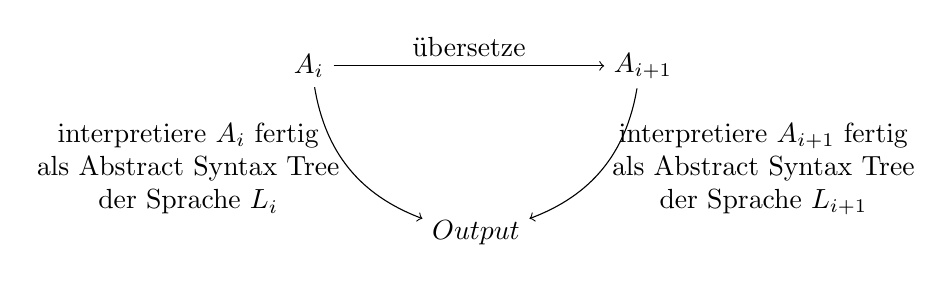
\begin{tikzpicture}[auto, baseline=(current  bounding  box.center)]
      \node (program1) at (135:3) {$A_{i}$};
      \node (program2) at (45:3) {$A_{i+1}$};
      \node (output)  at (270:0) {$Output$};

      % https://tex.stackexchange.com/questions/24372/how-to-add-newline-within-node-using-tikz
      \draw[->] (program1) to node[above] {übersetze} (program2);
      \draw[->] (program1) to[bend right] node[left, align=center] {interpretiere $A_{i}$ fertig\\ als Abstract Syntax Tree\\ der Sprache $L_{i}$} (output);
      \draw[->] (program2) to[bend left] node[right, align=center] {interpretiere $A_{i+1}$ fertig\\ als Abstract Syntax Tree\\ der Sprache $L_{i+1}$} (output);
    \end{tikzpicture}
    \label{eq:compiler_beziehungen}
  \end{equation}
  wobei man hier so tut, als gäbe es zwei \colorbold{Interpreter} für die zwei Sprachen $L_i$ und  $L_{i+1}$, welche den jeweiligen den \colorbold{Abstract Syntax Tree} $A_i$ bzw.  $A_{i+1}$ fertig interpretieren.\footnote{\colorbold{Interpretieren} geht immer von einem Programm in \colorbold{Konkretter Syntax} aus, wobei der \colorbold{Abstract Syntax Tree} ein \colorbold{Zwischenschritt} bei der \colorbold{Interpretierung} ist.}\footcite{g_siek_course_2022}
\end{Definition}

Die von den \colorbold{Passes} umgeformten \colorbold{Abstract Syntax Trees} sollten dabei mit jedem \colorbold{Pass} der \colorbold{Syntax} von \colorbold{RETI-Code} immer ähnlicher werden.

Jeder Pass sollte dabei möglichst \colorbold{eine} Aufgabe übernehmen, da der Sinn von \colorbold{Passes} ist, die Kompilierung in mehrere kleinschrittige Aufgaben runterzuberechen. Wie es auch schon der Zweck des \colorbold{Dervivation Tree} in der Syntaktischen Analyse war, eine Zwischenstufe zum \colorbold{Abstract Syntax Tree} darzustellen, aus der sich unkompliziert und einfach mit \colorbold{Transformern} und \colorbold{Visitors} ein \colorbold{Abstract Syntax Tree} generieren lies.

\begin{Definition}{Monadische Normalform}{monadische_normalform}
  Eine Sprache bei der
  \footcite{g_siek_course_2022}
\end{Definition}
\begin{Special_Paragraph}
  Ein echter Compiler verwendet Graph Coloring ... Register ...
\end{Special_Paragraph}

\section{Fehlermeldungen}
\begin{Definition}{Fehlermeldung}{fehlermeldung}
  \colorbold{Benachrichtigung} beliebiger Form, die darüber informiert, dass:
  \begin{enumerate}
    \item Ein Program beim \colorbold{Kompilieren} von der \colorbold{Konkretten Syntax} abweicht, also der \colorbold{Inpustring} sich nicht mit der Konrektten Syntax \colorbold{ableiten} lässt oder auf etwas \colorbold{zugegriffen} werden soll, was noch \colorbold{nicht} deklariert oder definiert wurde.
    \item Beim Ausführen eine \colorbold{verbotene} Operation ausgeführt wurde.\footcite{noauthor_errors_nodate}
  \end{enumerate}
\end{Definition}
\subsection{Kategorien von Fehlermeldungen}
